% !TEX encoding = UTF-8 Unicode
%!TEX root = ../Main/thesis.tex
% !TEX spellcheck = en-US
%%=========================================
\documentclass[../Main/thesis.tex]{subfiles}
\begin{document}
\chapter{Introduction}
\label{ch:introduction}
%The first chapter of a well-structured thesis is always an introduction, setting the scene with background, problem description, objectives, limitations, and then looking ahead to summarize what is in the rest of the report. 
%This is the part that readers look at first---\emph{so make sure it hooks them!}

%%=========================================
\section{Background}
\label{sec:background}
%In this section, you should present the problem that you are going to investigate or analyze; why this problem is of interest; what has, so far, been done to solve the problem, and which parts of the problem that remain.
%{\color{red}Below, I have set up some headings (subsection titles) without a number. 
%These are included to help you remember to cover the related issues. 
%The headings should be removed in your final print.}
%%=========================================
%\subsection*{Problem Formulation}
The associate press, a leading news organization, wrote: \say{Norwegian probe: Gearbox failure caused fatal 2016  crash}.
It was a news report of an airbus helicopter crash, on a small island outside of Bergen, the second largest city in Norway, cutting short the life of 13 people. The official cause of the crash: \say{A fatigue fracture in the main rotor gearbox.}. The anticipated question that arises after such catastrophic event is: was it preventable?
\justify
Since the industrial revolution, engines and machines have been the driving force for economic growth across industries such as automotive, airline, oil and gas, to name a few. However, machines are prone to failure, and must be monitored and maintained regularly, to avoid catastrophic failure, which can lead inevitably, to loss of human life and significant financial ruin. 
\justify
To mitigate equipment and machines proclivity toward failure and the associated cost, a process called predictive maintenance has been developed within the industrial community. Predictive maintenance  for machines and industrial equipment can be defined as a maintenance philosophy or more generally a framework, with a set of standards and methods, used to predict and prevent machine failure. This maintenance philosophy, when correctly implemented, increases machine life time, reduces downtime and maintenance cost. The aim here, is to detect as early as possible onset of failure and take appropriate actions.
\justify
In rotating machines such as gearboxes, more than $40 \% $ of failure can be attributed to bearing faults (\cite{albrecht1986}), as shown in figure \ref{fig:pie}, which displays the distribution of faults in rotating machines. By facilitating rotation movements, bearings can be subjected to large load and mechanical forces, which can lead to slowly propagating defects. The most commonly applied method in predictive maintenance for bearing faults detection, is a Fast Fourier Transform (FFT) based method. The latter consists of decomposing a vibration signal emanating from a bearing, to its corresponding frequency spectrum, through trigonometric basis functions. If the bearing exhibits signs of failure, the fundamental frequencies, which are the failure frequencies, will be consistently visible in the frequency spectrum. It is worth noting that, a bearing failure frequency is derived from its physical characteristics, and depends on the rotating speed of the machine housing the bearings.

\begin{figure}[H] %  figure placement: here, top, bottom, or page
   \centering
   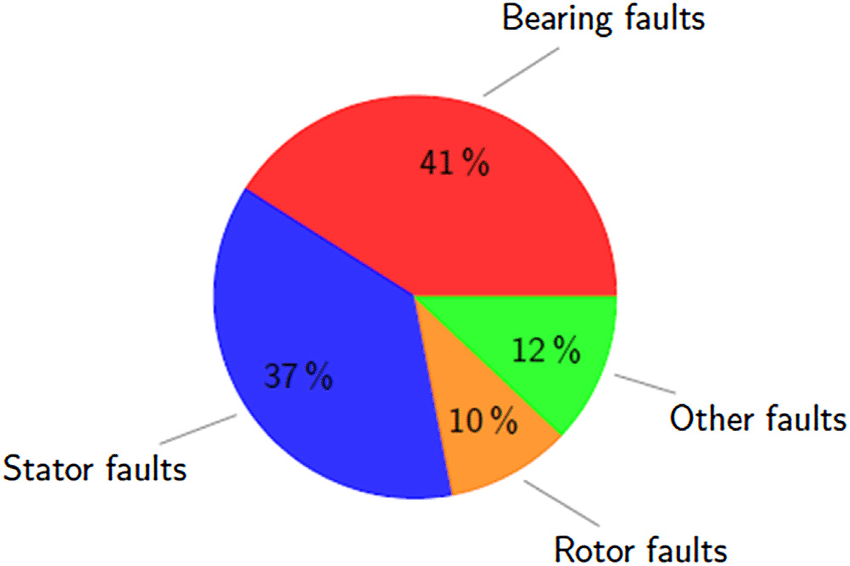
\includegraphics[width=4in]{../fig/pie.png} 
   \caption{Failure distribution in a rotating machine. }
   \label{fig:pie}
\end{figure}
\justify
The Fourier transform based method for bearing fault detection, although efficient, presents some limitations.
 For constant machine rotating speed, it is straight forward to estimate the fundamental frequencies. However, when the rotating speed varies continuously, it can be challenging to estimate the failure frequencies accurately, and this can lead to incorrect fault diagnosis. In addition, the trigonometric basis functions are not compactly supported, hence, an inability to capture local events in a signal.
\justify
To circumvent the latter, many efforts have been directed toward alternative methods for bearing fault detection. This thesis focuses on a method derived from Hilbert Huang transform. The latter, can reveal local phenomenon in a time signal, as opposed to Fourier transform based methods, that rely solely on the frequency spectrum.
\justify
Hilbert Huang transform was developed recently by  Huang, \cite{huang98} to deal efficiently with non linear and non stationary processes. It decomposes data adaptively 
into its sub-components by using the so called empirical mode decomposition (EMD). Unlike Fourier transform where trigonometric functions are used to decompose signals, adaptive decomposition means that 
the basis functions are completely determined by the data itself, \cite{huang08}. This allows in theory, to access intrinsic and salient properties of data
\justify
 The application of the aforementioned method for bearing failure detection, has been studied by various researchers. 
To set apart this work from what has been previously achieved, a literature survey is presented in section \ref{sec:relatedwork}. It starts by outlining Fourier analysis based methods, which rely on the fast Fourier transform or the short time Fourier transform, to obtain frequencies spectrum. Furthermore, some of the limitations of the Fourier analysis based methods are stressed out, and alternative techniques are lade out as mitigation. The contribution of this thesis is summarized in section \ref{sec:contributions}.
\justify
Since Fourier transform based methods are the standard for bearing fault detection across various industries, chapter \ref{sec:chapter2} shows how Fourier analysis is applied to bearing fault detection. In particular, the high frequency resonance technique (which will be discussed later) is applied to detect bearings failure. The chapter starts with an overview of Fourier series and Fourier transform, and later presents a case study in which, the high frequency resonance technique is used, to transform bearings vibration signals into frequencies spectrum, which contain bearing failure frequencies.
This will serve as a reference with regards to Hilbert Huang transform, wavelet transform and machine learning methods.
\justify
Chapters \ref{sec:hht} and \ref{sec:waveletandsvm} cover the contribution of this work. Chapter \ref{sec:hht} starts by showing how Hilbert Huang transform, coupled with a robust seasonal trend decomposition method, can detect high frequency and short duration pulses, generated by bearing faults. Chapter \ref{sec:waveletandsvm} on the other hand, presents a methodology to quantify bearings health, and classify multiple bearings with wavelet transform and machine learning. Chapter \ref{ch:conclusions} ends this thesis with a summary, pinpoint its limitations, and gives a road map to improve upon the latter.

%The detailed treatment of these methods and the 
%%=========================================
\clearpage
\section{Literature review}
\label{sec:relatedwork}
As part of nearly all rotating machines, rolling bearing elements are one of the most frequent reasons for machine breakdown (\cite{randal2010}). A rolling bearing element is made of mainly four parts, which are shown in Figure \ref{fig:bearing-s}: The outer race indicated by 1, the balls trapped in the cage and labeled by 2 and 3 respectively. Finally, the inner race identified by 4 and 5. To facilitate machine rotation, a rotating shaft, which is a long cylindrical tube, is placed within the inner ring.
\begin{figure}[H]
	\centering
	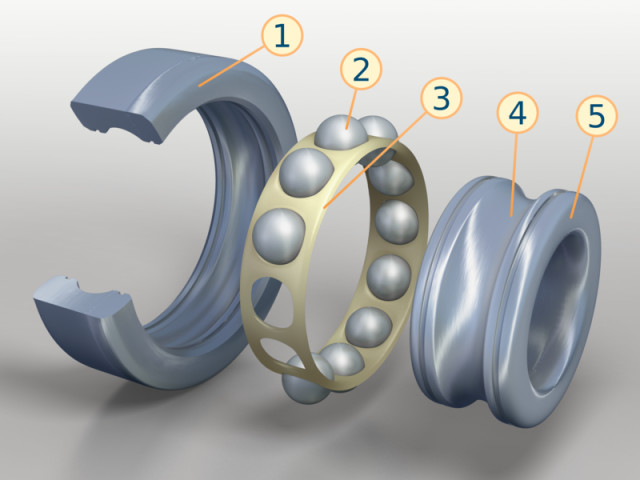
\includegraphics[width=0.5\linewidth]{../fig/bearing-s}
	\caption{Exploded view of a rolling bearing. 1: outer race or ring, 2: balls or roller elements, 3: cage, 4 and 5: inner race or ring.}
	\label{fig:bearing-s}
\end{figure}
\justify
Premature and unexpected bearing breakdown, can halt production and incur high cost. In the worst case scenario, human lives can be impacted. To avert dramatic consequences of bearing failure, it is therefore crucial to detect incipient faults and take appropriate actions.
\justify
The geometry of a bearing is important in understanding its dynamic, and detecting early sign of failure.
 A key fact in bearing fault detection, is that a failure can be detected at a given frequency, called characteristic defect frequency or failure frequency. Here is why. A defect in one surface of a rolling element bearing also called balls, generates an impulse as it hits an other surface, (\cite{mcfadden1984a}, \cite{mcfadden1984b}). As the bearing rotates, the impulses will occur periodically with a frequency (the defect frequency) which is uniquely determined by the location of the defect (\cite{mcfadden1984a}). Consequently, the failure frequency is derived from the bearing physical characteristics, and the rotational speed of the machine housing the bearing, (\cite{mcfadden1984a}). Therefore, finding the failure frequencies is the basis for bearing fault detection in most cases.
%and can be found in the vibration signal frequency spectrum it generates. 
%The latter is obtained by transforming the vibration signal with a mathematical transformation such as Fourier transform. 
\justify
There are typically four failure frequencies: ball pass frequency outer race (BPFO), which is the frequency at which a defect strikes the outer ring. Similarly, the ball pass frequency inner race (BPFI) is the frequency at which a defect hits the inner race. The fundamental train frequency cage (FTF) and the ball spin frequency (BSF) are frequencies at which a fault tricks the cage and the rollers (balls), respectively.
\justify
Finding the failure frequencies entails, transforming the bearing vibration signal into its corresponding frequency spectrum, where the defect frequencies reside. However, this apparent simple task is challenging. The vibration signal of a bearing is \say{infected} by the signals of other machines components or other vibration sources (\cite{zhao2014}, \cite{mcfadden1984a}). In addition, at the onset of failure, the fault frequencies are very weak (\cite{zhao2014}). To efficiently detect failure frequencies, a de-noising of the signal is necessary and the weak early defect frequencies must be enhanced (\cite{zhao2014}). 
\justify
To address the aforementioned issues, several signal processing techniques have been proposed. The most prevalent are (\cite{zhao2014}): the high frequency resonance technique (HFRT) (\cite{darlow1974}), Spectral kurtosis (\cite{antoni2006a}, \cite{antoni2006b}, \cite{antoni2007}), wavelet analysis (\cite{lin2000}, \cite{qiu2006}), Hilbert Huang transform and the empirical mode decomposition (\cite{yu2005}, \cite{lei2011}), cyclostationary approach (\cite{antoni2004}, \cite{borghesani2013}, \cite{girondin2013}), minimum entropy deconvolution (\cite{sawalhi2007}, \cite{jiang2013} ), and stochastic resonance (\cite{tan2009}, \cite{he2012}). The most widely used method is however the high resonance frequency technique, because it is able to efficiently extract bearing diagnostic information, trough a sequence of filtering operations (\cite{zhao2014}).
%In addition, under harsh conditions such as time varying machine rotational speed and load or large shock, the vibration signals are low signal noise ration and non stationary \cite{zhao2014}.

\justify
One of the first work on bearing fault detection was by (\cite{balderston1969}), who investigated bearings rings and roller elements (balls) natural frequencies, and observed that the signal induced by bearings defects are located in the high frequency zone of resonance exited by the internal impact of the faults, (\cite{randal2010}). Let elaborate on this. As previously mention, a bearing defect will generate periodic impulses, which are forces that strike the bearing at the location of the defect, at a given frequency (failure frequency). When the failure frequency is equal, or nearly equal to the natural frequency of the bearing, this cause the latter to vibrate at a higher amplitude and frequency (\cite{mcfadden1984a}), then it would have at a different frequency. This phenomenon is called mechanical resonance. The latter will also occur in the machine housing the bearing, and in a potential sensor mounted on the bearing for collecting vibration data, (\cite{mcfadden1984a}).
\justify
 It is therefore critical to detect, and isolate the resonance exited by the impulses generated by bearing defects, which in theory can be visible in the bearing vibration signal. However, bearing diagnostic information in the form of failure frequencies are  difficult to be directly observable in the raw signal (\cite{randal2010}). This is due to the fact that the energy generated by the impulses induced by faults, are widely distributed over a wide range of frequencies (\cite{randal2010}).
 \justify
 To circumvent the latter difficulty, the high frequency resonance technique (HFRT) was developed and  allowed early detection of bearing failure (\cite{broderick1972}, \cite{burchill1973}, \cite{burchill1973b}, \cite{darlow1974}, \cite{darlow1975}, \cite{darlow1975b}, \cite{board1975},  \cite{randal2010}, \cite{gupta2016}, \cite{khadersab2018}).
In the high frequency resonance technique, a bearing vibration signal is  band pass filtered, envelop-detected, low pass filtered and finally decomposed into its frequency spectrum by the Fourier transform.
\justify
 The resonance induced by defects, are responses of the bearing, the machine housing the bearing, and possibly other surrounding machines (\cite{mcfadden1984a}). Therefore band pass filtering allows only the bearing signal to be recovered.
 The envelop detection procedure, extracts the high frequency resonance signal produced by the bearing defects. This signal is the superposition of two components: the high frequency resonance component and the low frequency bearing failure component. The latter is recovered by a low pass filter. 
 \justify
  Recall that a band pass filtering process in signal processing, filters a signal by only letting through desire frequencies. On the other hand, the envelop detection process, takes a target signal and returns its envelope. The latter is the curve formed by joining all peaks in the signal. In practice, the envelope signal is derived by taking the Hilbert transform of the band pass filtered signal. The low pass filter procedure, sips out low frequency components of a signal.
\justify
The diagnostic power of the high frequency resonance technique rests on the key fact that it uses the envelope of the band passed raw vibration signal, before performing the Fourier transform (\cite{mcfadden1984a}, \cite{randal2010}). The envelope signal contains nearly all the information generated by bearing faults. It is worth noting that the rollers elements located in the bearing cage are subjected to random slip, (\cite{mcfadden1984a}), and the bearing failure frequencies variation is of the order of 1-2$\%$ (\cite{randal2010}). This random slip changes the characteristics of the raw vibration signal, which makes it difficult to extract useful diagnostic information directly from the vibration raw signal, (\cite{randal2010}). However, the sequence of operation applied to the raw signal to obtain the envelope addresses specifically this situation of slip  (\cite{randal2010}). 
\justify
The envelope signal obtained from the High frequency resonance technique was also leveraged in other methods for bearing fault detection. For example, the spectral kurtosis method, uses the frequency spectrum of the envelope signal from the short time Fourier transform (STFT), to find the frequency band of the pulses generated by bearing fault (\cite{randal2010}). The spectral kurtosis uses fourth order statistical moment, to decompose the power of a signal with respect to frequencies, (\cite{randal2010}). Note that the short time Fourier transform uses fixed window size where the Fourier transform is applied. Akin to the spectral kurtosis, is the power spectral density (PSD) method, which uses second order statistics, to obtain the energy contribution of frequencies. The bearing failure frequency will generally produce a larger energy distribution.
% The random slip induce a fundamental change in the raw signal rendering it stochastic and makes it inefficient for bearing fault detection, \cite{randal2010}. 
\justify
 Although powerful, the high frequency resonance technique can produce a noisy spectrum for inner race or rolling element defect (\cite{mcfadden1984a}). The spectrum can become even more noisy when bearing defects are extensive (\cite{mcfadden1984a}). The dependency of the failure frequency on the machine rotation speed, can also be an issue as the rotating speed changes continuously or is unknown. Time varying rotation speed and load can cause the vibration signal to be non-stationary (\cite{zhao2014}), which makes the Fourier transform inadequate (\cite{huang98}, \cite{huang08}).
 \justify
  In addition, the Fourier transform uses trigonometric basis functions, that are not locally compact, and can not handle efficiently nonlinear and non-stationary signal (\cite{huang98}). The reader might argue that the short time Fourier transform, can handle non-stationary signal. However, the issue in this case is the selection of the window size. An other important issue for all frequency based method so far mentioned, are the selection of a resonance frequency band for band pass filtering the raw vibration signal (\cite{zhao2014}). The resonance frequency band, is the frequency band within which, the frequencies of resonance induced by the faults are located.
 \justify
 
 
\justify
 To extend bearing fault detection to cases where a Fourier transform based method or more generally frequency based methods are limited,
numerous contributions have been made towards alternative methods such as Hilbert Huang transform, wavelet transform and machine learning (\cite{zhang2019}, \cite{xiaoan2018}, \cite{rai2016}, \cite{konar2011}, \cite{rai2006} ). These methods can directly operate in the time domain (on the time signal), as opposed to Fourier transform based methods that require a frequency spectrum. 
\justify
The Hilbert Huang transform (HHT) as most signal analysis tool, is predicated on the key assumption that a signal has multiple components, and can be decomposed into single oscillatory modes called intrinsic mode functions (IMFs) (\cite{fosso2019}, \cite{huang08}, \cite{huang98}). It was developed to deal efficiently with nonlinear and non-stationary signals. As opposed to Fourier transfrom, the HHT method does not use a-priori basis functions. It uses local properties of a signal such as the extrema of a signal, the mean, with a series of operations to obtain a hierarchy of single component signals, that range from high to low frequency time signals. By using local properties, the HHT is able to model local events such as pulses emitted by bearing faults (which will be shown in this thesis). The wavelet transform on the other hand, utilizes locally compact basis functions, and was primarily used in geophysics, to model high frequency short duration seismic pulses, (\cite{albert09}), similar to those emitted by bearing faults .
\justify
For bearing fault detection, (\cite{fan2016}) decomposed the vibration signal obtained from a motor into intrinsic mode functions, and evaluated the Hilbert Huang energy spectrum (also called marginal spectrum) of each IMF, to detect sign of fatigue, oxidation and mechanical structure deformation. In the same fashion (\cite{peng2004}, \cite{soualhi2015}, \cite{osman2014},\cite{osman2013a}, \cite{osman2013b}, \cite{li2008}) Applied the marginal spectrum to identify bearing characteristic defect frequencies. The energy spectrum also called power spectrum or energy density, is the energy contribution of each frequency, derived from the intrinsic mode functions.
To compute the energy density, the Hilbert transform of the absolute value of the square of an IMF is first computed. Secondly, the integral of the latter is evaluated over the domain of variability of the signal. The Hilbert transform of a signal is the convolution of the signal with the function $\frac{1}{\pi t}$, where $t$ is a dummy variable.
\justify
One of the issue of the Hilbert Huang transform, is selecting the appropriate intrinsic mode functions (\cite{fosso2019}). The IMFs obtained from a target signal, are hierarchy of mono component signals, ranging from high to low frequency. However, due to a phenomenon called mode mixing, an IMF, rather then having a single oscillatory mode, can have more than one mode, resulting an IMF to lose its physical meaning (\cite{fosso2019}). For a given process such as the vibration of a bearing in a motor, there exists multiple sub processes corresponding to the vibration of sub components of the motor and the bearing. Therefore mapping the correct IMFs to the corresponding sub processes is a daunting task.
\justify
 To resolve this issue, (\cite{osman2013a}, \cite{osman2013b} ) used a linear combination of two similarities measure (Linear and non-linear similarity) to select the target IMF and applied the energy spectrum of the IMFs to identify bearing failure frequencies. The similarities measures, quantifies the \say{sameness} of two distributions.
In the same fashion (\cite{osman2014}) applied a weighted D'Agostino Pearson (DP) normality test to select the more relevant IMFs (IMF representing defect component). The DP test uses both the skewness and the kurtosis to assess normality.
The skewness is a statistical estimator that measures the symmetry of a probability distribution, while the kurtosis also a statistical estimator, measures the \say{tailedness} of a distribution. The Kurtosis and skewness of a normal distribution are 3 and 0 respectively. (\cite{peng2004}), used the correlation coefficient as a criteria for IMF selection.
\justify
A large majority of Hilbert Huang transform methods applied to bearing fault detection uses the energy spectrum of the IMFs to identify the bearing failure frequencies (more citation here)
\justify
 




%%=========================================

\section{Contributions }
\label{sec:contributions}
This thesis introduces a complementary method for bearing fault detection. Most industrial bearing detection method use the Hight frequency resonance technique or its derivation. This methods rely on a series of signal filtering and the Fourier transform to obtain a frequency spectrum. Due to the inability of the Fourier transform to deal efficiently with frequency or amplitude modulated signal, the resulting spectrum can be noisy. In this thesis, the Hilbert Huang transform is coupled with a robust seasonal decomposition method for bearing fault detection. The Hilbert Huang transform decomposes a bearing vibraton signal into nearly mono component signals. Furthermore, the seasonal part of the signal. 
\justify
%
% coupled with a one class support vector machine to classify a system of bearing into healthy and unhealthy classes.


%%=========================================

\blankpage
\end{document}
